\documentclass[DIV=calc, paper=a4, fontsize=11pt]{scrartcl}


\usepackage{makeidx}
\usepackage{graphicx}
\usepackage{flushend}

\usepackage{lmodern}
\usepackage[left=1.5cm,right=1.5cm,top=2.5cm,bottom=2cm]{geometry}
\usepackage{float}		
\bibliographystyle{plain} 
\pagestyle{plain} 
\pagenumbering{arabic}
\usepackage{fancyhdr} 	


\usepackage[T1]{fontenc}
\usepackage[utf8]{inputenc}
\usepackage[spanish]{babel}
\usepackage{hyperref}
\usepackage{graphicx}

\usepackage{lipsum}
\usepackage[protrusion=true,expansion=true]{microtype}
\usepackage{amsmath,amsfonts,amsthm}
\usepackage[svgnames]{xcolor}
\usepackage[svgnames]{xcolor}
\usepackage{booktabs}
\usepackage{fix-cm}
\usepackage{multicol}
\newenvironment{Figura}
  {\par\medskip\noindent\minipage{\linewidth}}
  {\endminipage\par\medskip}

\usepackage{sectsty}
\allsectionsfont{\usefont{OT1}{phv}{b}{n}}

\usepackage{fancyhdr}
\pagestyle{fancy}
\usepackage{lastpage}

\lhead{}
\chead{}
\rhead{}

\lfoot{}
\cfoot{}
\rfoot{\footnotesize Page \thepage\ of \pageref{LastPage}}

\renewcommand{\headrulewidth}{0.0pt}
\renewcommand{\footrulewidth}{0.4pt}

\usepackage{lettrine}
\newcommand{\initial}[1]{\lettrine[lines=3,lhang=0.3,nindent=0em]{
\color{DarkGoldenrod}{\textsf{#1}}}{}}

\usepackage{titling}

\newcommand{\HorRule}{\color{DarkGoldenrod} \rule{\linewidth}{1pt}}

\pretitle{\vspace{-120pt} \begin{flushleft} \HorRule \fontsize{22}{35} \usefont{OT1}{phv}{b}{n} \color{DarkRed} \selectfont}

\title{Ley de enfriamiento de Newton\\ %Aquí va el nombre de la práctica 
Práctica 3} %Numero de la práctica 

\posttitle{\par\end{flushleft}\vskip 0.5em}

\preauthor{\begin{flushleft}\large \lineskip 0.5em \usefont{OT1}{phv}{b}{sl} \color{DarkRed}}

\author{Misael Iván Macías Márquez\\
misaelmacias@ciencias.unam.mx}

\postauthor{\footnotesize \usefont{OT1}{phv}{m}{sl} \color{Black}

\vspace*{0.1cm} Facultad de Ciencias, UNAM

\par\end{flushleft}\HorRule}

\date{Martes 22 de Marzo de 2022\\Semestre 2022-1}


\begin{document}

\maketitle


\begin{abstract}
\textbf{Resumen:} Se comprobó que el enfriamiento de un cuerpo inmerso en un medio a menor temperatura cumple con la ley de enfriamiento de Newton es decir que la temperatura es proporcional a la exponencial del tiempo (ver ecuación 4), el ajusto por exponencial dio un coeficiente de correlación $R^2 = 0.97$ por lo que se concluye que la relación anterior se cumple.


\end{abstract}

\begin{multicols}{2}




\section*{Introducción}

La ley del enfriamiento de Newton o enfriamiento newtoniano establece que la tasa de pérdida de calor de un cuerpo es proporcional a la diferencia de temperatura entre el cuerpo y sus alrededores. Cuando la diferencia de temperaturas entre un cuerpo y su medio ambiente no es demasiado grande, el calor transferido en la unidad de tiempo hacia el cuerpo o desde el cuerpo por conducción, convección y radiación es aproximadamente proporcional a la diferencia de temperatura entre el cuerpo y el medio externo[1].

$\\$

Cuando la diferencia de temperaturas entre un cuerpo y su medio ambiente no es demasiado grande, el calor transferido en la unidad de tiempo hacia el cuerpo o desde el cuerpo por conducción, convección y radiación es aproximadamente proporcional a la diferencia de temperatura entre el cuerpo y el medio externo[2].

\begin{equation}
    \frac{d Q}{dt} = -r (T-T_m)
\end{equation}

 \noindent donde $T$ es la temperatura y $T_m$ la temperatura ambiente.Si la temperatura T del cuerpo es mayor que la temperatura del medio ambiente Ta, el cuerpo pierde una cantidad de calor dQ en el intervalo de tiempo comprendido entre t y t+dt, disminuyendo su temperatura T en dT[2].
\begin{equation}
    d Q = m c dT
\end{equation}

\noindent donde $m$ es la masa y $c$ el calor específico, entonces sustituyendo la ecuación 2 en la 1


\begin{equation*}
    \frac{m c dT}{dt} = -r (T-T_m) 
\end{equation*}

\begin{equation}
    \frac{dT}{dt} = -\frac{r}{mc} (T - T_m) = -k (T - T_m)
\end{equation}

\noindent con $k=r/mc$, entonces integrando la ecuación 3 de la temperatura $T_0$ a $T$ y del tiempo $0$ a $t$ 

\begin{equation*}
    \int_{T_0}^{T} \frac{dT}{T-T_m} = -k \int_{0}^{t} dt
\end{equation*}

\begin{equation*}
    \ln{(T-T_m)} = -kt+ \ln{(T_0 - T_m)}
\end{equation*}

\noindent y despejando $T$

\begin{equation}
    T  -T_m= (T_0 - T_m) e^{-kt} 
\end{equation}







\section*{Desarrollo experimental}

Se llenó el recipiente de aluminio con agua de grifo para después colocarlo en la hornilla de la estufa antes de encender la ornílla, con el termómetro digital se determinó la temperatura ambiente $T_m$ del cuarto, ya con la hormilla encendida se dejó calentar el agua por un par de minutos hasta alcanzar una temperatura inicial $T_0$, posteriormente se vertió el agua calentada en el vaso de unicel para después con el termómetro y el cronometro  medir la temperatura $T$ del agua cada 2 min.


\begin{Figura}
    \centering
    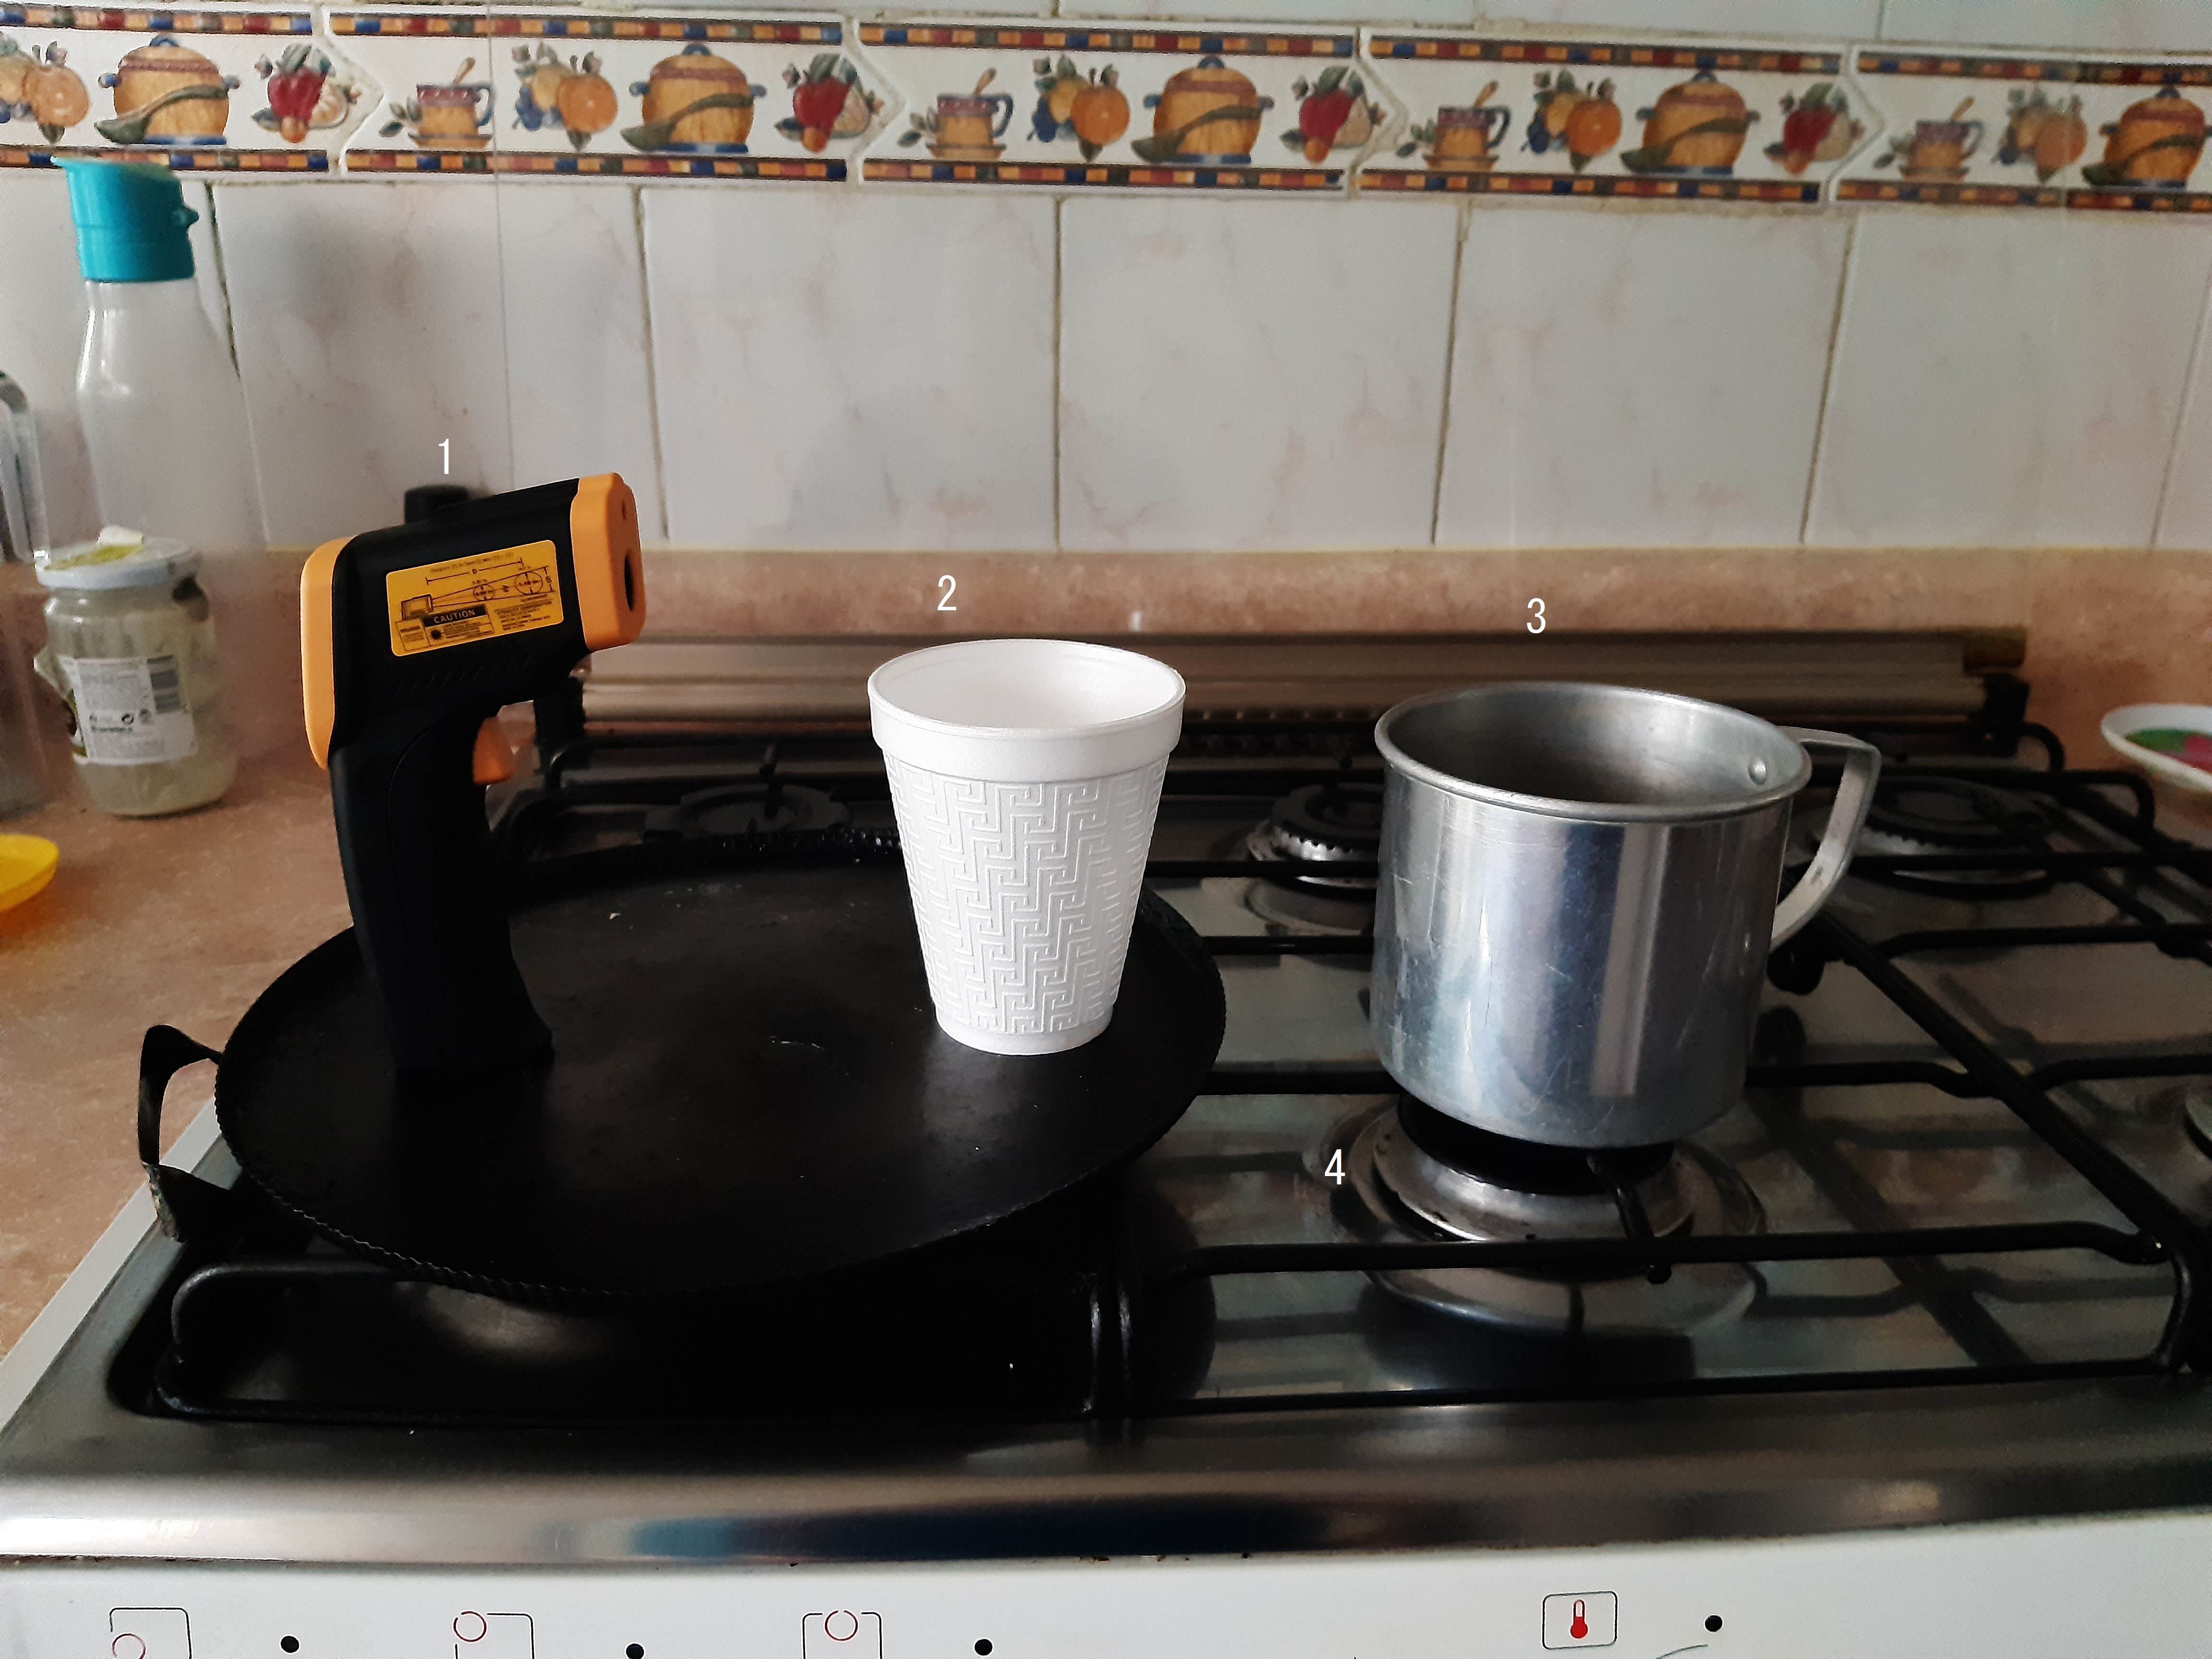
\includegraphics[width=0.9\textwidth]{20220224_162210.jpg}
    \captionof{figure}{Arreglo experimental:(1) Termómetro digital, (2) Vaso de unicel, (3) recipiente de aluminio, (4) hornilla de estufa}
    \label{fig}
\end{Figura}






\section*{Resultados y Análisis}

Las temperaturas medidas y sus respectivos tiempos se pueden encontrar en la figura 3 (ver anexos), la temperatura ambiente es:

\begin{equation*}
    T_m = 22.5 ^\circ C
\end{equation*}



\noindent entonces restando a la temperatura medida la temperatura ambiente para graficar la función mostrada en la ecuación 4 y ajustando por una exponencial tenemos que:



\begin{Figura}
    \centering
    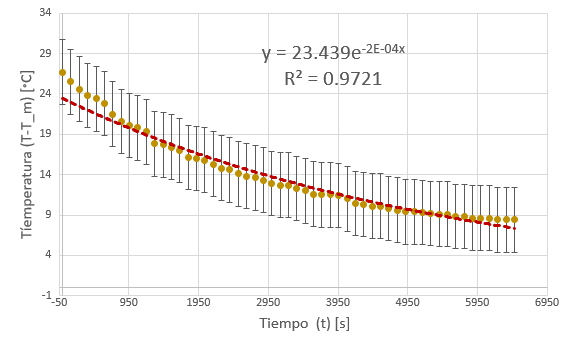
\includegraphics[width=1.1\textwidth]{grafica newton.PNG}
    \captionof{figure}{Gráfica del ajuste por exponencial para los datos de la figura 3 aplicando la ecuación 4}
    \label{fig}
\end{Figura}

\noindent donde el coeficiente de correlación $R^2$ es aproximadamente $0.97$.



\section*{Conclusiones}

Al tenerse un coeficiente de correlación $R^2$ tan cercano al 1 se puede concluir que la relación dada por la ecuación 4 sí describe el comportamiento de un cuerpo enfriándose a temperatura $T$ inmerso en un medio a temperatura $T_m$ con $T> T_m$.


  
\begin{thebibliography}{99}

\bibitem{1} “Ley Del Enfriamiento de Newton.” 2020. Wikipedia. Marzo 18, 2020. https://es.wikipedia.org/wiki/Ley\_del
\_enfriamiento\_de\_Newton.

\bibitem{2} “Ley Del Enfriamiento de Newton.” n.d. Www.sc.ehu.es. http://www.sc.ehu.es/sbweb/fisica/estadistica
/otros/enfriamiento/enfriamiento.htm.

\bibitem{3} Oda, Berta. Introducción al análisis gráfico de datos experimentales. 3a ed. Ciudad de México: las prensas de ciencias, 2017.

\end{thebibliography}








\end{multicols}

\newpage

\section*{Apéndices}

\begin{figure}[h!]
    \centering
    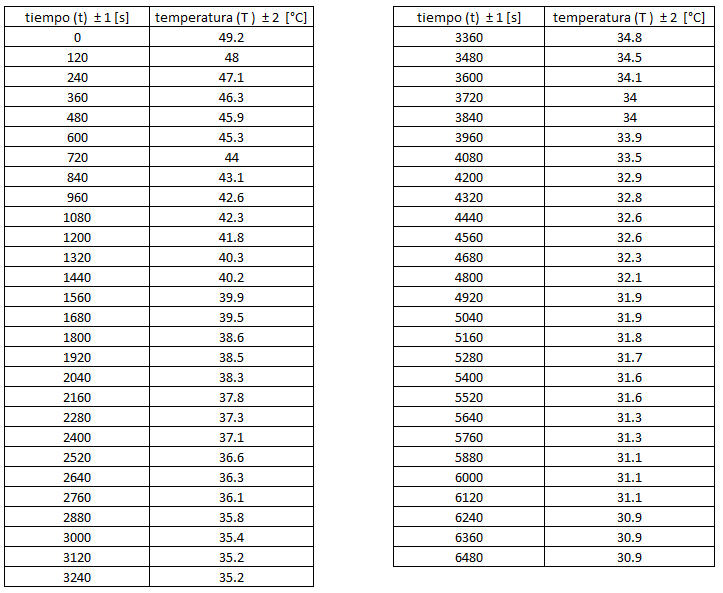
\includegraphics[scale=0.8]{tabla newton.PNG}
    \caption{Tiempos y temperaturas medidas.}
    \label{fig:my_label}
\end{figure}
\end{document}